\section{Experimental Results and Evaluation}
\label{sec:evaluation}

\subsection{Overall Model Comparison on Locked Out-of-Time Test}
Table~\ref{tab:oot_results} presents the single-pass benchmark of our Development-frozen candidate models on the unseen Locked Out-of-Time (OOT) Test cohort ($N = 50{,}653$, $25.59\%$ default rate), and Figure~\ref{fig:oot_roc_pr} plots their corresponding ROC and Precision--Recall curves.

\begin{table}[htbp]
  \centering
  \caption{Model performance on the Locked OOT Test Set (\texttt{F2\_safe}, $N = 50{,}653$, $25.59\%$ default rate).}
  \label{tab:oot_results}
  \footnotesize
  \setlength{\tabcolsep}{4.5pt}
  \begin{tabular}{@{}lcccccr@{}}
    \toprule
    \textbf{Model} & \textbf{Dev CV AUC} & \textbf{OOT AUC} & \textbf{PR-AUC} & \textbf{KS} & \textbf{F1@Opt ($\tau$)} & \textbf{Fit (s)} \\
    \midrule
    \textbf{\texttt{LightGBM} (Tuned)} & $0.6748$ & $\mathbf{0.6621}$ & $\mathbf{0.3910}$ & $0.2368$ & $\mathbf{0.4540}$ ($0.205$) & $10.9$ \\
    \texttt{XGBoost} (Tuned) & $\mathbf{0.6749}$ & $0.6620$ & $0.3907$ & $\mathbf{0.2369}$ & $0.4526$ ($0.209$) & $13.3$ \\
    \texttt{RandomForest} (Base) & $0.6688$ & $0.6554$ & $0.3820$ & $0.2275$ & $0.4505$ ($0.205$) & $8.9$ \\
    \texttt{LogisticRegression} ($C=0.1$) & $0.6653$ & $0.6525$ & $0.3762$ & $0.2232$ & $0.4516$ ($0.192$) & $\mathbf{1.7}$ \\
    \texttt{MLP} (128, 64) & $0.6658$ & $0.6525$ & $0.3770$ & $0.2221$ & $0.4475$ ($0.195$) & $7.5$ \\
    \texttt{DecisionTree} (Base) & $0.6389$ & $0.6270$ & $0.3501$ & $0.1905$ & $0.4306$ ($0.195$) & $3.4$ \\
    \bottomrule
  \end{tabular}
\end{table}

\begin{figure}[htbp]
  \centering
  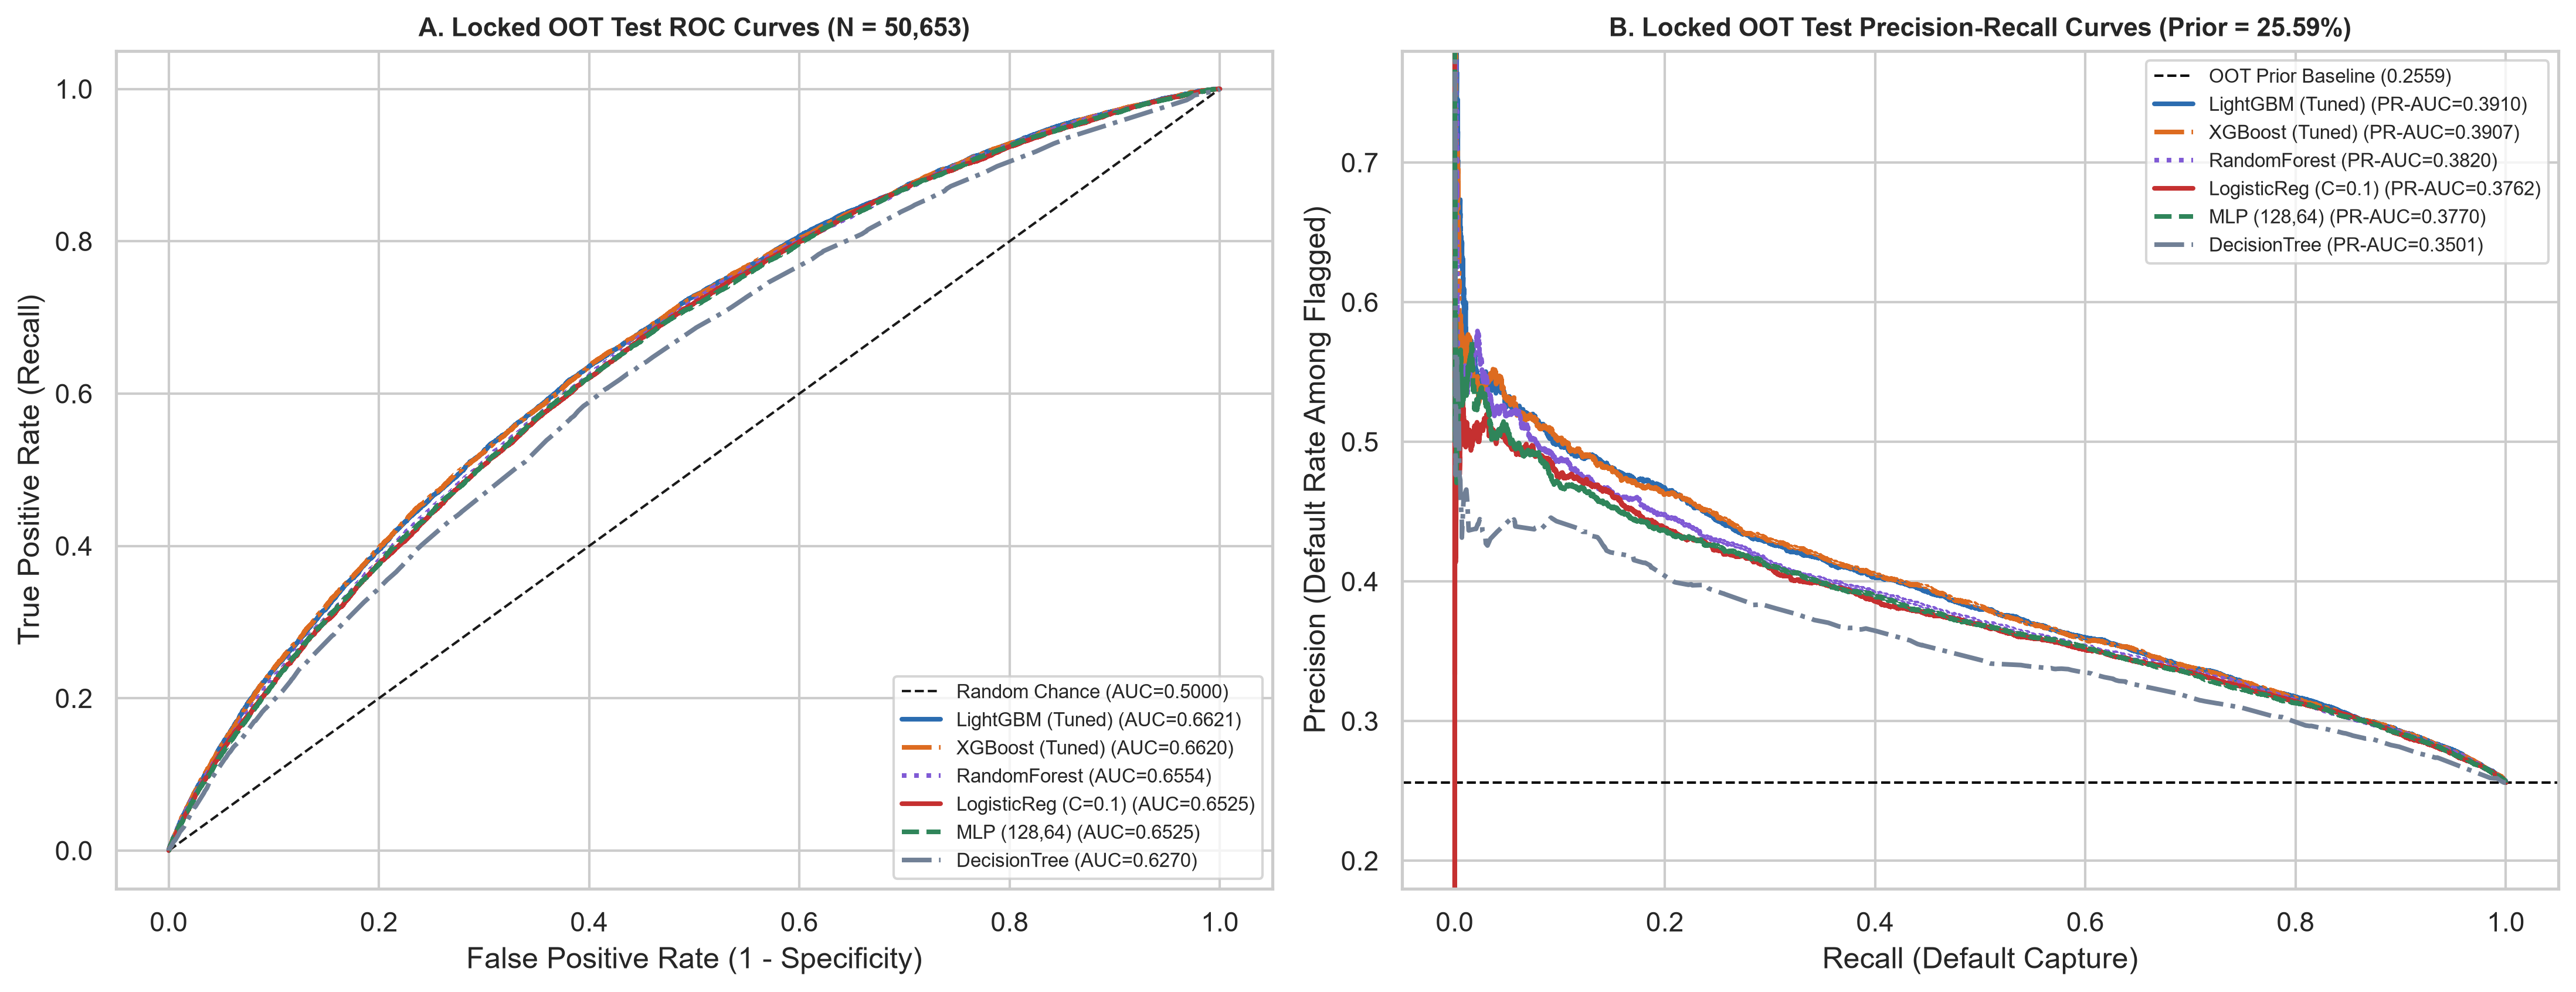
\includegraphics[width=0.95\textwidth]{figures/final_01_oot_roc_pr_curves.png}
  \caption{Out-of-Time ROC curves (left) and Precision--Recall curves relative to the $0.2559$ test baseline (right) on $N = 50{,}653$ contracts.}
  \label{fig:oot_roc_pr}
\end{figure}

Three clear findings stand out from Table~\ref{tab:oot_results}. First, the two tuned GBDT models lead all paradigms almost identically---\texttt{LightGBM} ($\text{OOT AUC} = 0.6621$, $\text{PR-AUC} = 0.3910$) and \texttt{XGBoost} ($0.6620$, $\text{PR-AUC} = 0.3907$)---achieving a $1.53\times$ Precision--Recall lift over the $0.2559$ test base rate. Second, both GBDTs clearly outperform \texttt{RandomForest} ($0.6554$, $-0.0067$ AUC), \texttt{LogisticRegression} ($0.6525$, $-0.0096$ AUC), the \texttt{MLP} baseline ($0.6525$), and the single \texttt{DecisionTree} ($0.6270$). Third, consistent with tabular benchmarks~\cite{gunnarsson2021,grinsztajn2022}, the controlled \texttt{MLP} baseline ($0.6525$, Brier $0.1834$, ECE $0.0573$) offers no ranking advantage over \texttt{LogisticRegression} ($0.6525$, ECE $0.0490$) while running $4.4\times$ slower ($7.5\text{ s}$ vs.\ $1.7\text{ s}$) and exhibiting weaker calibration. \texttt{LightGBM} is therefore selected as the primary champion model due to top OOT ranking, fast training time ($10.9\text{ s}$), strong Development probability calibration ($\text{ECE} = 0.0017$), and exact millisecond TreeSHAP attribution.

\subsection{Impact of Feature Engineering and Validation Strategy}
To evaluate how engineered features transfer to future contracts and how random train-test splitting distorts evaluation, Table~\ref{tab:fe_and_split} compares feature tiers on OOT Test alongside Stratified Random $80/20$ versus Locked OOT validation, illustrated visually in Figure~\ref{fig:rq3_split}.

\begin{table}[htbp]
  \centering
  \caption{Feature engineering ablation across tiers (Panel A) and Random 80/20 vs.\ Locked OOT validation bias (Panel B).}
  \label{tab:fe_and_split}
  \scriptsize
  \setlength{\tabcolsep}{3.0pt}
  \begin{tabular}{@{}llccccc@{}}
    \toprule
    \multicolumn{7}{@{}l}{\textbf{Panel A: Feature Tier Ablation on Locked OOT Test (ROC-AUC, $N = 50{,}653$)}} \\
    \midrule
    \textbf{Tier} & \textbf{Feature Additions} & \textbf{\texttt{LR}} & \textbf{\texttt{LGBM}} & \textbf{\texttt{XGB}} & \textbf{Avg.\ Gain vs.\ \texttt{F0}} & \\
    \midrule
    \texttt{F0} & Cleaned raw + 3 parsed fields & $0.6319$ & $0.6483$ & $0.6478$ & --- & \\
    \texttt{F1} & $+$29 domain ratios \& bureau split & $0.6345$ & $0.6506$ & $0.6500$ & $+0.0023$ & \\
    \textbf{\texttt{F2\_safe}} & \textbf{$+$ \texttt{branch}, \texttt{supplier}, \texttt{pincode}} & $\mathbf{0.6525}$ & $\mathbf{0.6621}$ & $\mathbf{0.6620}$ & $\mathbf{+0.0162}$ & \\
    \texttt{F2\_plus\_emp} & $+$ \texttt{Employee\_code\_ID} & $0.6543$ & $0.6636$ & $0.6635$ & $+0.0178$ & \\
    \midrule
    \multicolumn{7}{@{}l}{\textbf{Panel B: Stratified Random 80/20 vs.\ Locked OOT Validation on \texttt{F2\_safe}}} \\
    \midrule
    \textbf{Model} & \textbf{Rand.\ AUC} & \textbf{OOT AUC} & \textbf{Opt.\ Bias} & \textbf{Rand.\ ECE} & \textbf{OOT ECE} & \textbf{ECE Infl.} \\
    \midrule
    \texttt{LightGBM} (Tuned) & $0.6713$ & $\mathbf{0.6621}$ & $+0.0091$ & $\mathbf{0.0016}$ & $0.0491$ & $+0.0475$ ($30\times$) \\
    \texttt{XGBoost} (Tuned) & $\mathbf{0.6717}$ & $0.6620$ & $+0.0097$ & $0.0026$ & $\mathbf{0.0489}$ & $+0.0463$ ($19\times$) \\
    \texttt{RandomForest} (Base) & $0.6660$ & $0.6554$ & $+0.0106$ & $0.0128$ & $0.0499$ & $+0.0371$ ($4\times$) \\
    \texttt{LogisticReg.} ($C=0.1$) & $0.6629$ & $0.6525$ & $+0.0103$ & $0.0068$ & $0.0490$ & $+0.0421$ ($7\times$) \\
    \bottomrule
  \end{tabular}
\end{table}

\begin{figure}[htbp]
  \centering
  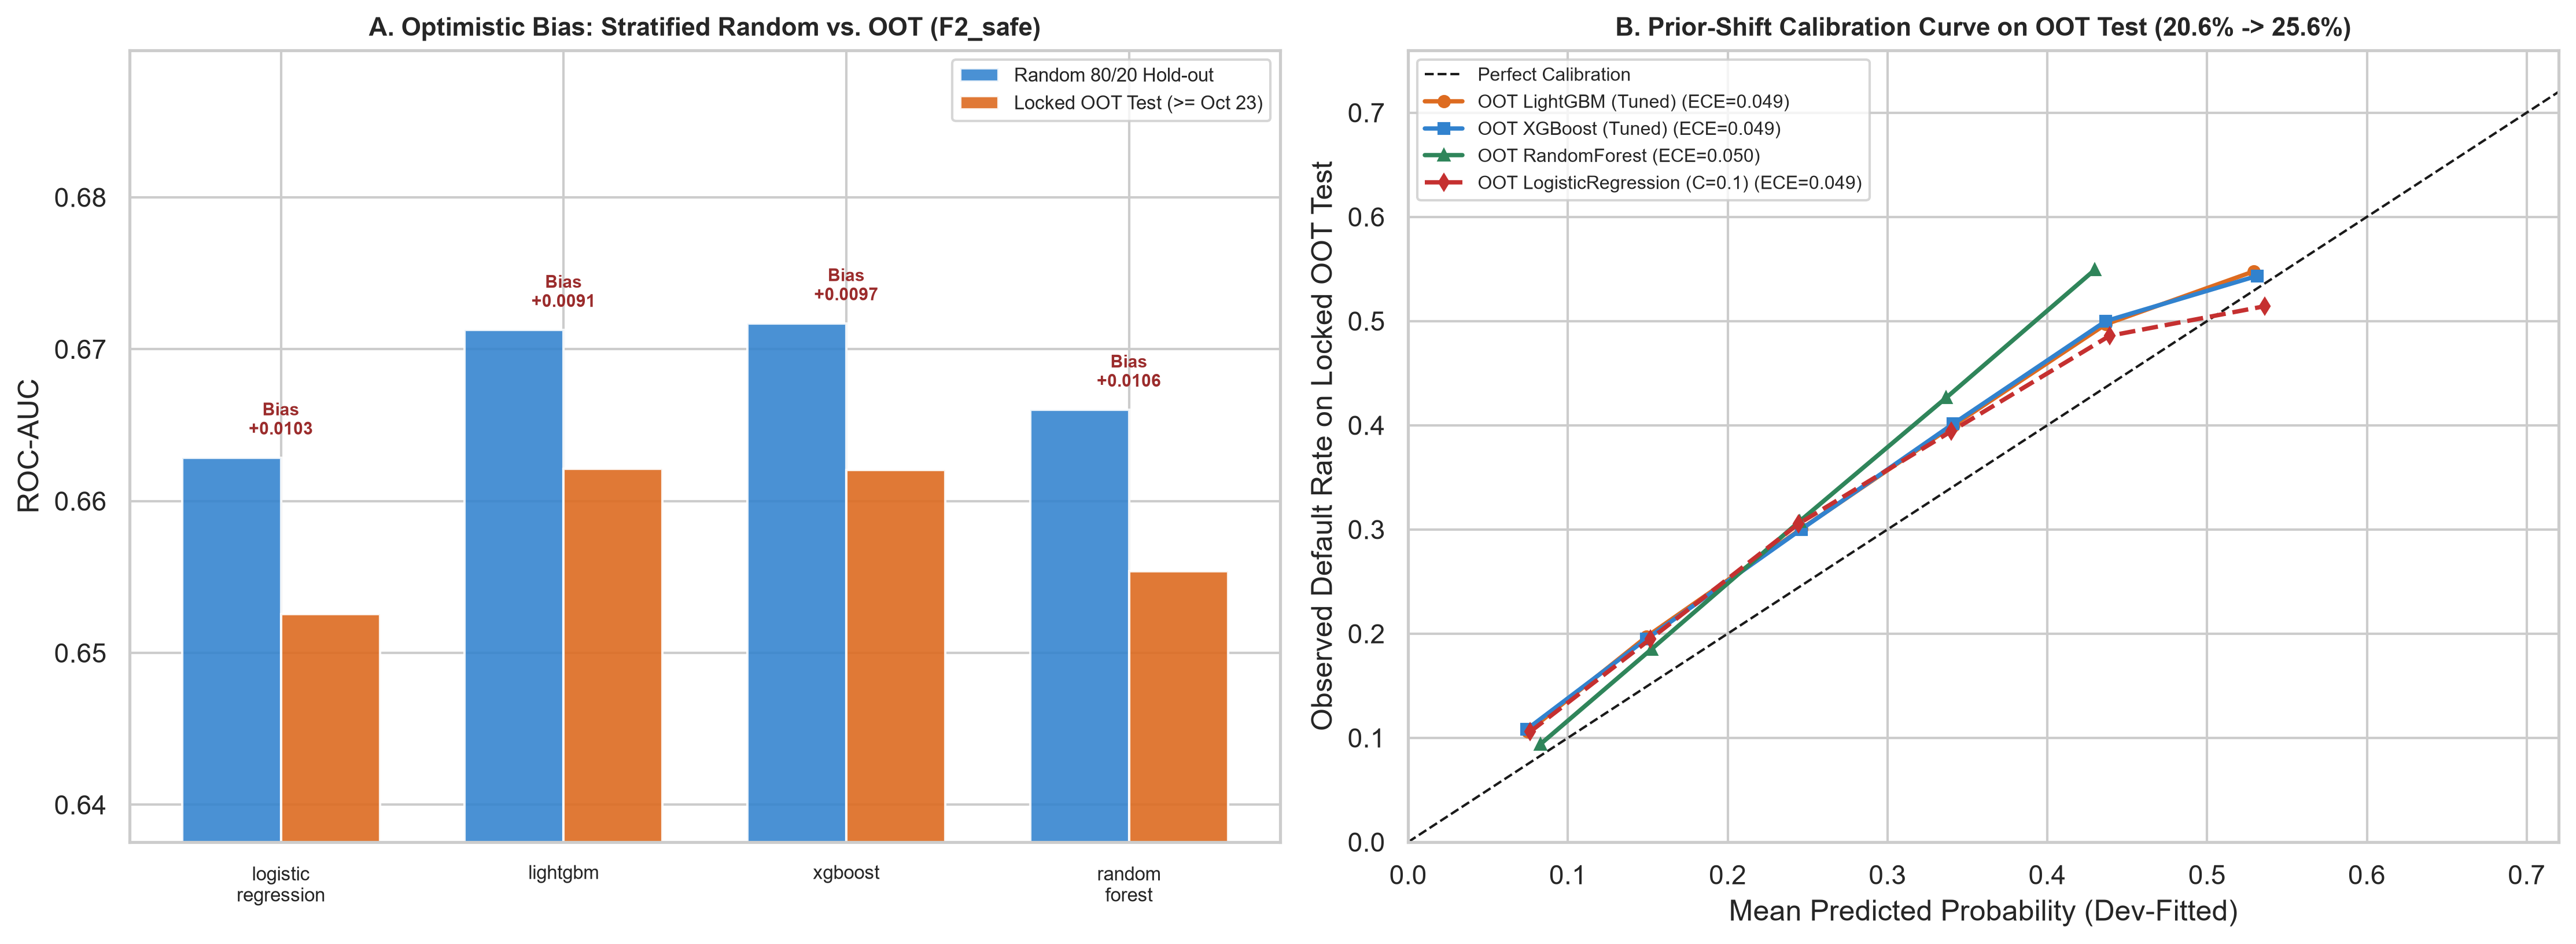
\includegraphics[width=0.95\textwidth]{figures/final_02_oot_vs_random_rq3.png}
  \caption{Comparison of Stratified Random splitting vs.\ Locked OOT Test: ROC-AUC optimism bias (left) and calibration curve shift caused by higher late-October default rates (right).}
  \label{fig:rq3_split}
\end{figure}

In Panel~A, domain financial engineering (\texttt{F0 -> F1}) delivers steady gains across all models ($+0.0021\text{--}+0.0026$ AUC), confirming the value of isolating non-scored bureau codes ($<300$) and adding leverage ratios. Introducing fold-safe OOF target encoding for dealer, branch, and postal channels (\texttt{F1 -> F2\_safe}) yields the largest leap ($+0.0115\text{--}+0.0180$ AUC) despite entity cold-start rates of $0.00\%$ on \texttt{branch\_id}, $0.80\%$ on \texttt{supplier\_id}, and $0.85\%$ on \texttt{Current\_pincode\_ID}. Adding \texttt{Employee\_code\_ID} (\texttt{F2\_plus\_emp}) adds $+0.0015$ short-term AUC over the 9-day October test window, yet suffers the highest unseen cold-start rate ($0.99\%$) and staff-turnover sensitivity, making \texttt{F2\_safe} safer for deployment.

Panel~B exposes two critical validation traps in standard random splitting. First, 80/20 Stratified Random evaluation artificially inflates ROC-AUC by $+0.0091$ to $+0.0106$ because uniform sampling shares same-day promotional cohorts and dealer clusters across train and test. Second, Random splitting reports nearly perfect probability calibration for LightGBM ($\text{ECE} = 0.0016$), hiding a $30$-fold ECE jump ($0.0491$) when default prevalence climbs from $20.63\%$ to $25.59\%$. As Figure~\ref{fig:rq3_split} (right) shows, every model's OOT reliability curve shifts parallel and roughly $5\text{ percentage points}$ above the diagonal, underscoring the need for temporal testing and periodic base-rate recalibration.

\subsection{Class Imbalance and Decision Threshold Analysis}
Table~\ref{tab:imbalance_thresh} evaluates six fold-isolated class-imbalance treatments (Panel~A) and five Development-frozen decision thresholds (Panel~B) on Stage-2 \texttt{LightGBM}. Figures~\ref{fig:imbalance_ablation} and~\ref{fig:thresholds} visualize the feature-ablation/imbalance contrast and the probability threshold trade-offs.

\begin{table}[htbp]
  \centering
  \caption{Imbalance correction strategies (Panel A) and Dev-frozen threshold transfer (Panel B) for Stage-2 \texttt{LightGBM} on Locked OOT Test ($N = 50{,}653$).}
  \label{tab:imbalance_thresh}
  \scriptsize
  \setlength{\tabcolsep}{3.5pt}
  \begin{tabular}{@{}lcccccc@{}}
    \toprule
    \multicolumn{7}{@{}l}{\textbf{Panel A: Fold-Isolated Imbalance Treatments on Locked OOT Test}} \\
    \midrule
    \textbf{Strategy} & \textbf{Train $N$} & \textbf{ROC-AUC} & \textbf{PR-AUC} & \textbf{Brier} & \textbf{ECE} & \textbf{Fit (s)} \\
    \midrule
    \textbf{\texttt{natural} ($\text{weight}=1.0$)} & $182{,}501$ & $0.6621$ & $0.3910$ & $\mathbf{0.1810}$ & $0.0491$ & $10.2$ \\
    \texttt{mild\_weight\_2.0} & $182{,}501$ & $\mathbf{0.6623}$ & $\mathbf{0.3912}$ & $0.1845$ & $0.0729$ & $10.7$ \\
    \texttt{class\_weight} ($\approx 3.85$) & $182{,}501$ & $0.6620$ & $0.3909$ & $0.2257$ & $\mathbf{0.2111}$ & $10.0$ \\
    \texttt{RUS 0.5} & $112{,}947$ & $0.6613$ & $0.3897$ & $0.1839$ & $0.0676$ & $\mathbf{7.3}$ \\
    \texttt{SMOTE 0.5} & $217{,}278$ & $0.6446$ & $0.3612$ & $0.1843$ & $0.0372$ & $18.1$ \\
    \texttt{SMOTE 1.0} & $289{,}704$ & $0.6252$ & $0.3453$ & $0.2013$ & $0.0977$ & $22.3$ \\
    \midrule
    \multicolumn{7}{@{}l}{\textbf{Panel B: Transfer of Pre-Frozen Operating Thresholds onto Locked OOT Test}} \\
    \midrule
    \textbf{Policy ($\tau_{\text{Dev}}$)} & \textbf{Flagged (\%)} & \textbf{Appr.\ (\%)} & \textbf{Prec.\ (\%)} & \textbf{Recall (\%)} & \textbf{F1-Score} & \textbf{Amt Loss (\%)} \\
    \midrule
    \texttt{Default} ($\tau = 0.500$) & $0.64$ & $99.36$ & $\mathbf{56.5}$ & $1.4$ & $0.0274$ & $13.12$ \\
    \texttt{Capacity Top-20\%} ($0.293$) & $20.18$ & $79.82$ & $42.0$ & $33.1$ & $0.3700$ & $9.95$ \\
    \texttt{Bayes 3:1} ($0.250$) & $31.38$ & $68.62$ & $38.6$ & $47.4$ & $0.4255$ & $8.78$ \\
    \texttt{F1-Optimal} ($0.205$) & $45.97$ & $54.03$ & $35.3$ & $63.5$ & $0.4540$ & $7.69$ \\
    \textbf{\texttt{Bayes 5:1} ($0.167$)} & $59.39$ & $40.61$ & $32.6$ & $\mathbf{75.6}$ & $\mathbf{0.4555}$ & $\mathbf{7.13}$ \\
    \bottomrule
  \end{tabular}
\end{table}

\begin{figure}[htbp]
  \centering
  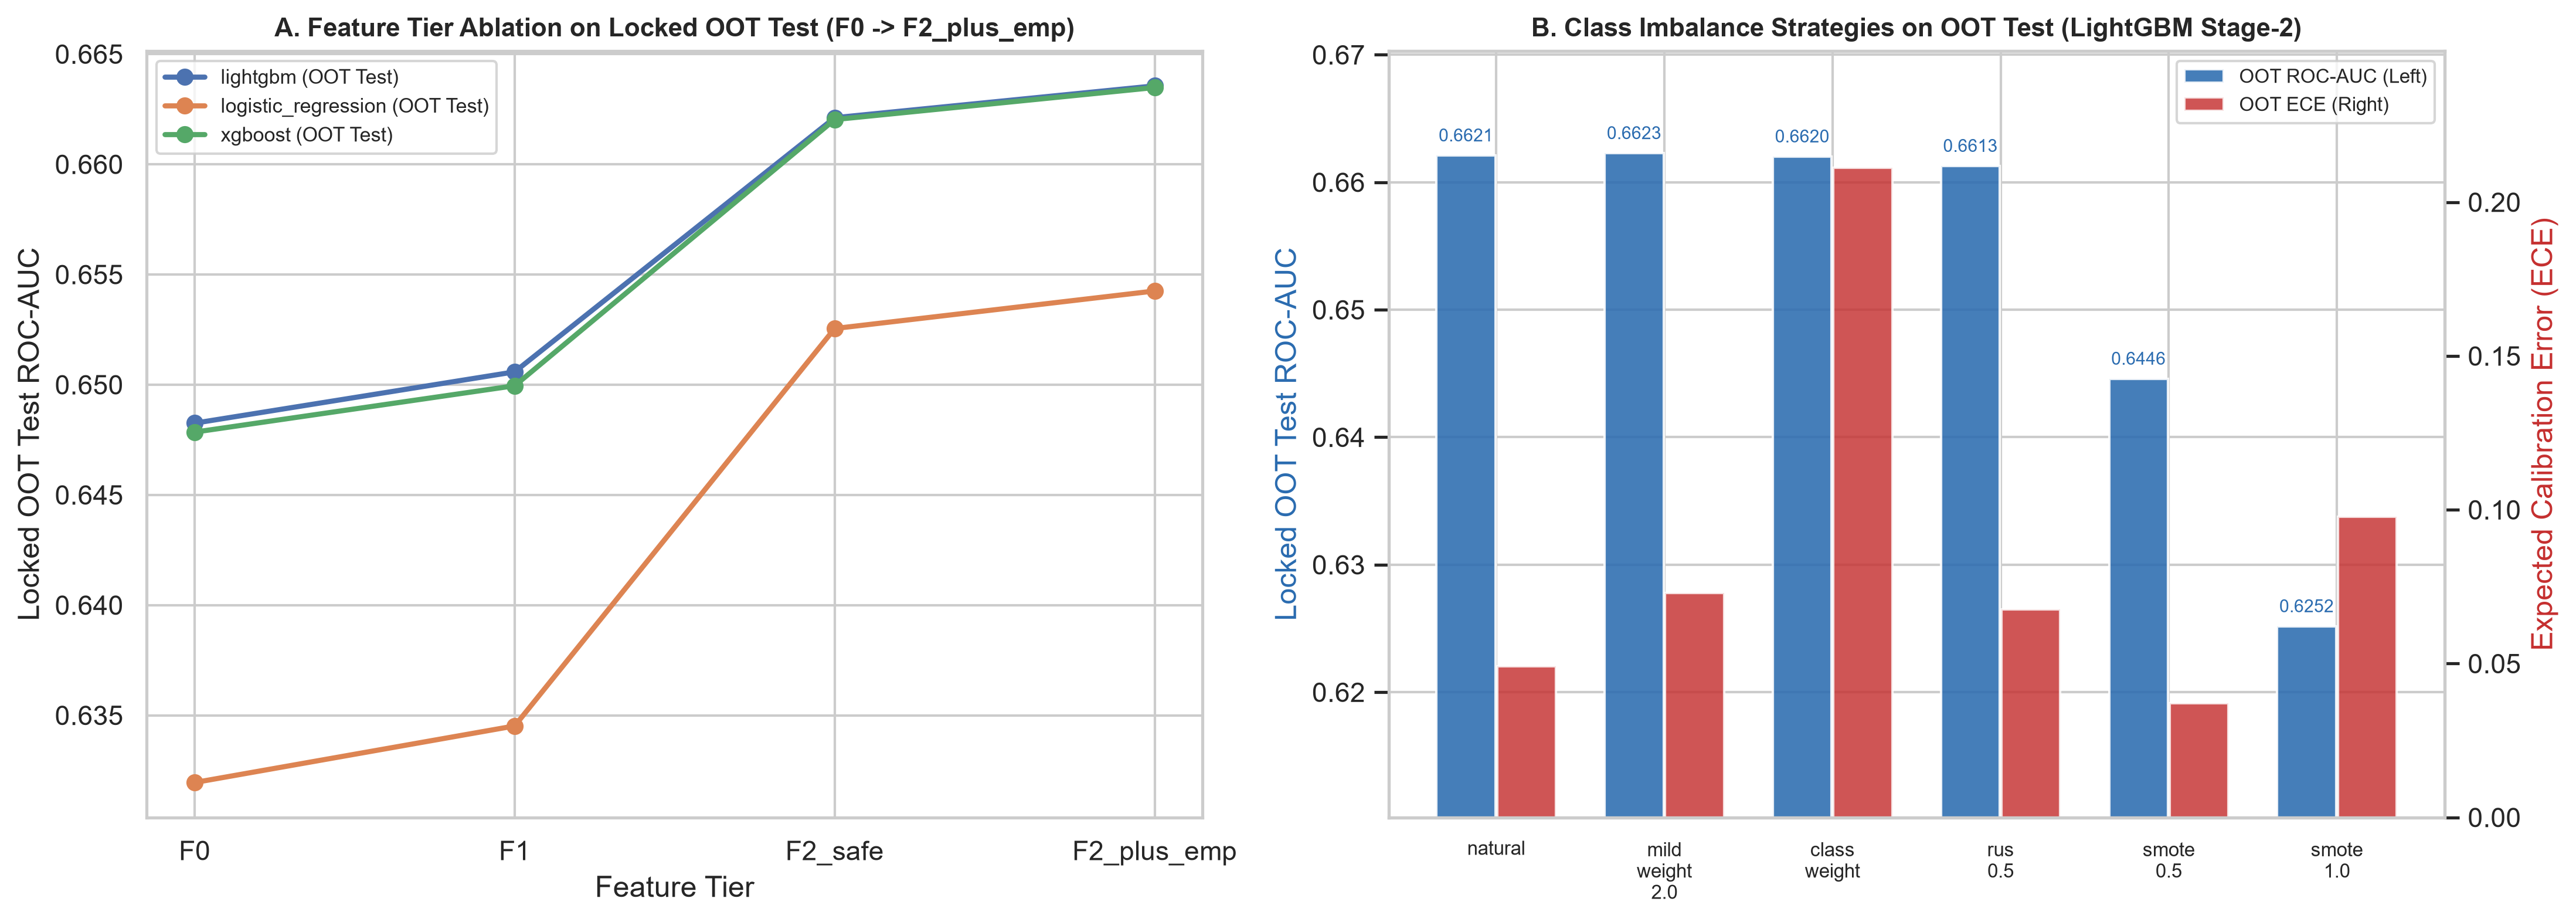
\includegraphics[width=0.95\textwidth]{figures/final_03_rq2_ablation_oot_and_imbalance.png}
  \caption{Out-of-Time feature tier progression (left) and fold-isolated imbalance performance confirming sharp SMOTE degradation on LightGBM (right).}
  \label{fig:imbalance_ablation}
\end{figure}

\begin{figure}[htbp]
  \centering
  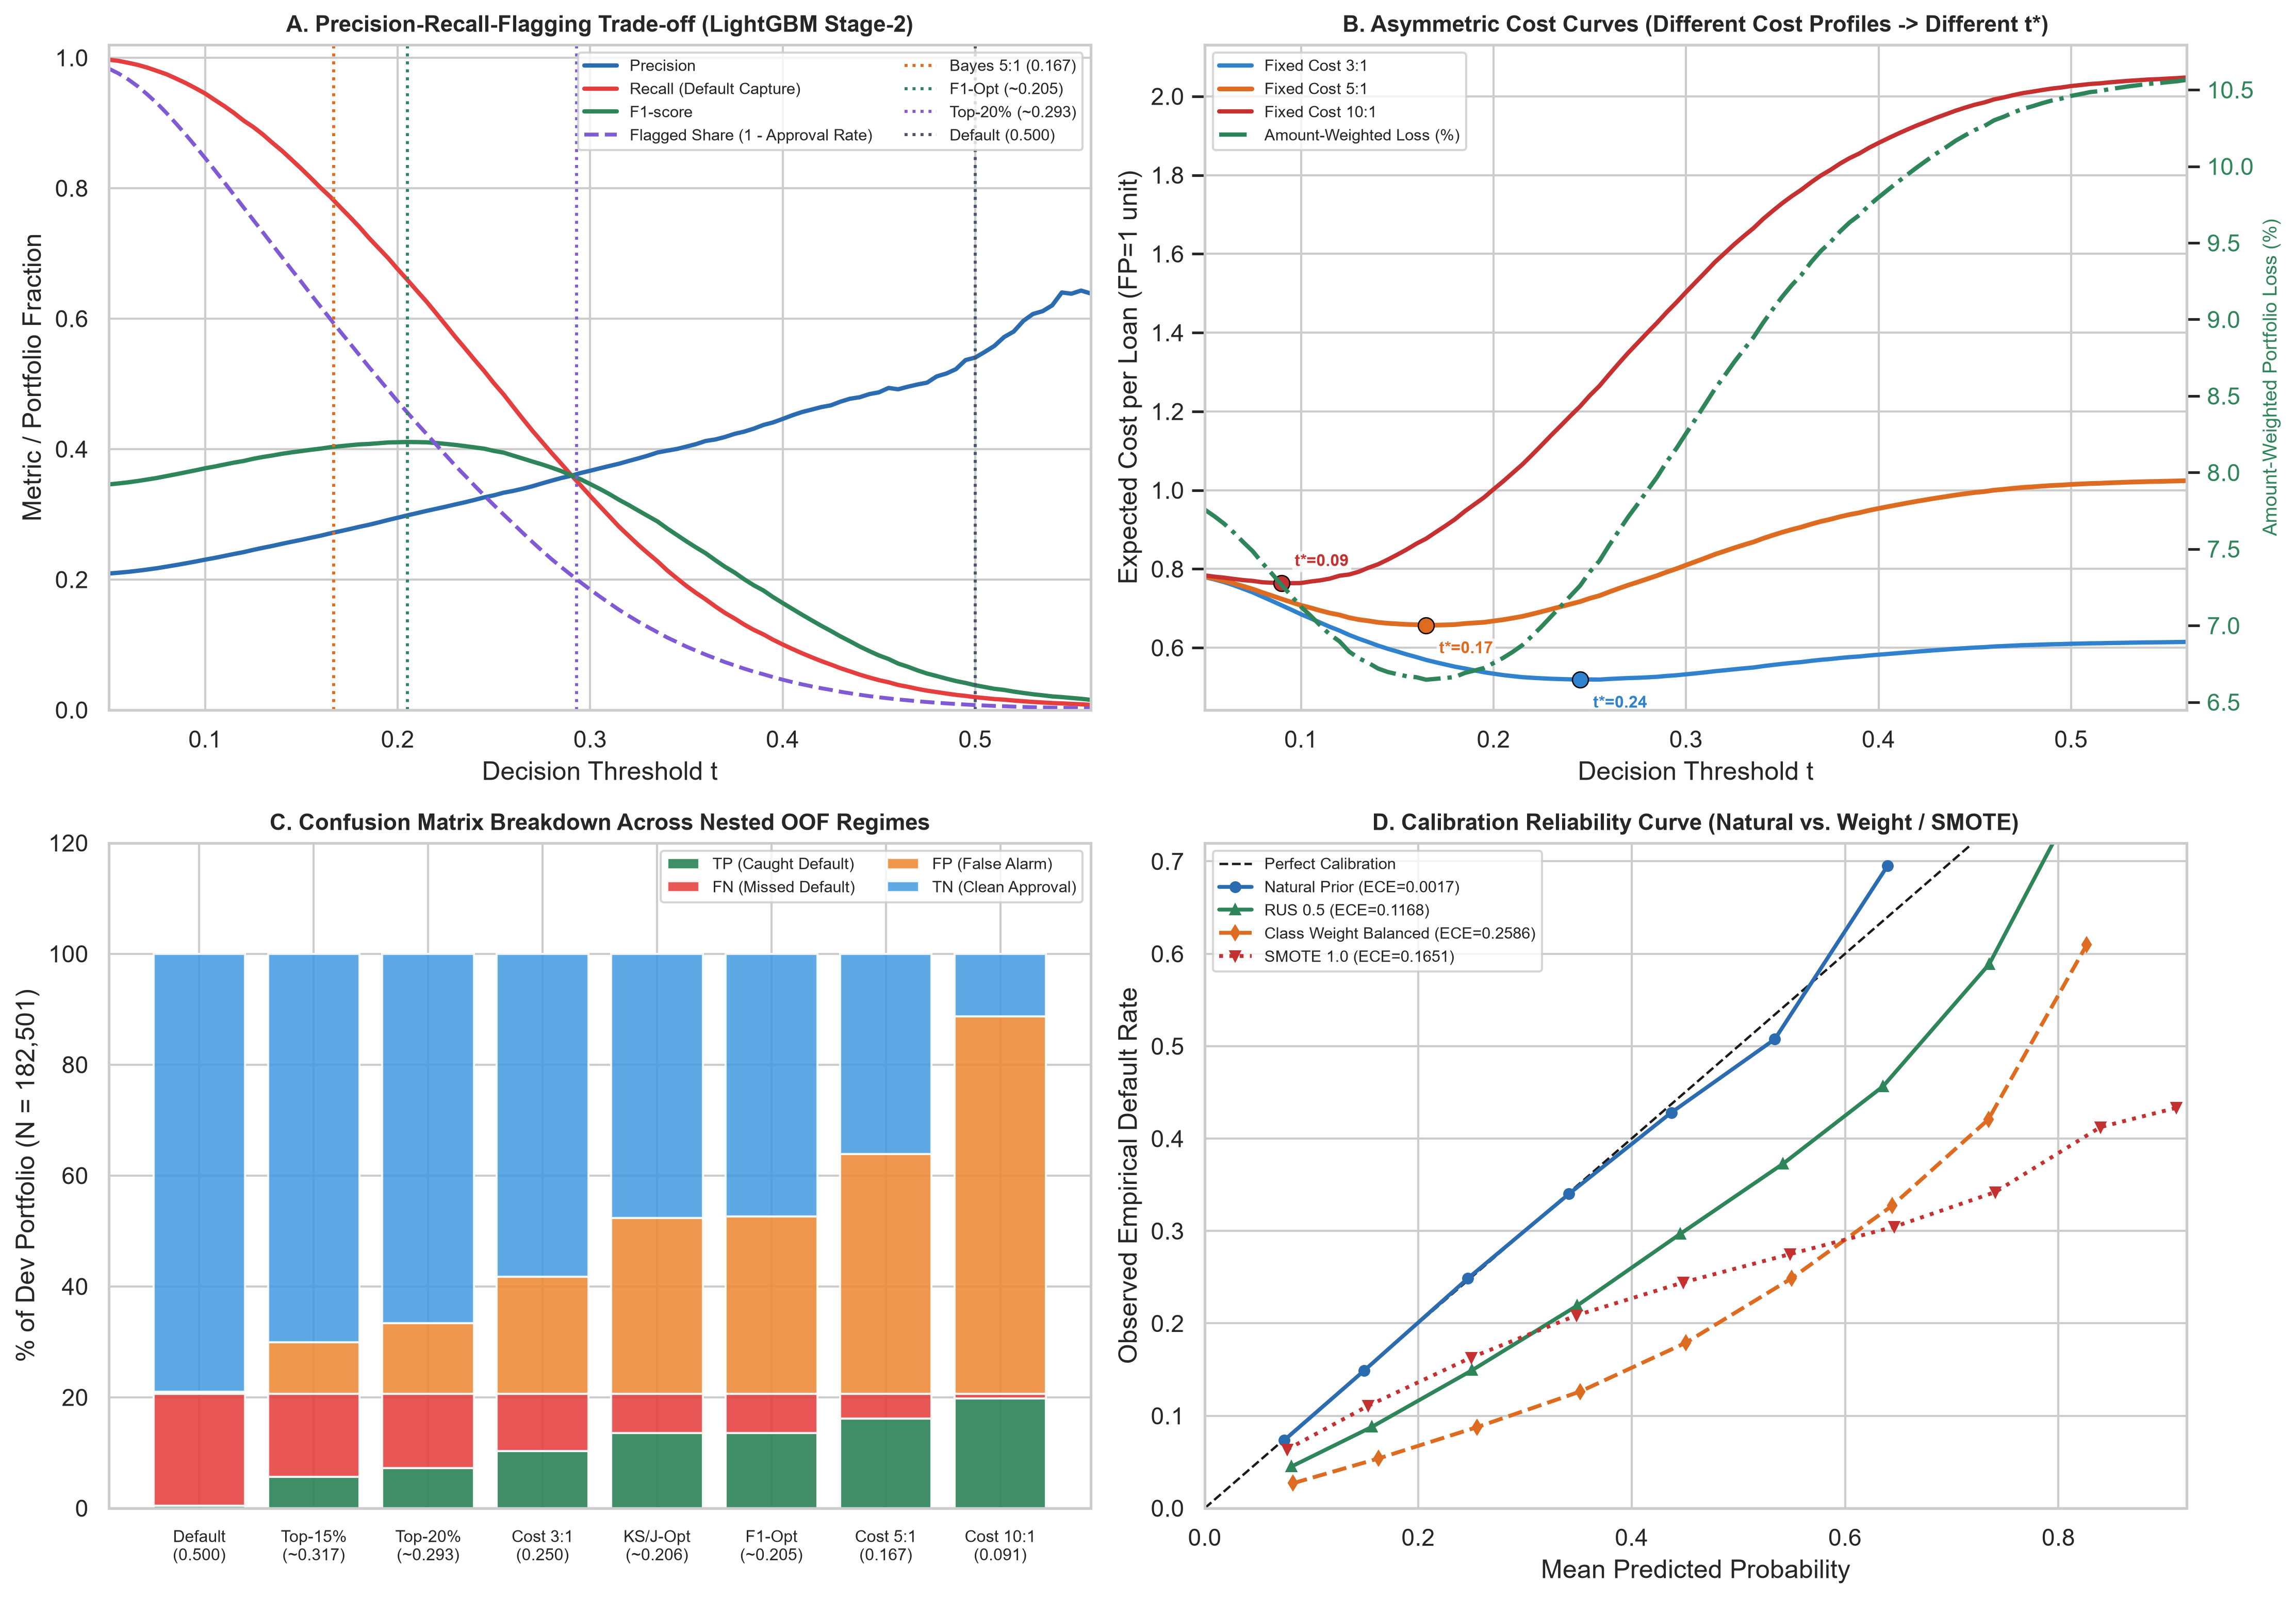
\includegraphics[width=0.95\textwidth]{figures/opt_01_threshold_tradeoffs.png}
  \caption{Threshold policy trade-offs across approval rate, recall, precision, portfolio financial loss, and calibration curves evaluated via nested 5-fold Development OOF.}
  \label{fig:thresholds}
\end{figure}

Three practical lessons emerge clearly. First, \textbf{strictly fold-isolated SMOTE actively harms GBDTs}: at ratio $1.0$, \texttt{SMOTE} drops LightGBM OOT ROC-AUC by $-0.0369$ ($0.6621 \to 0.6252$) and PR-AUC by $-0.0456$. This happens because linear Euclidean interpolation across a $123$-column matrix containing dozens of binary KYC flags and one-hot categories creates unrealistic fractional synthetic points between $0$ and $1$, causing trees to overfit artificial split boundaries. Notably, \texttt{SMOTE 0.5} exhibits a lower raw OOT ECE ($0.0372$) than \texttt{natural} ($0.0491$) only because SMOTE's upward probability inflation (Dev ECE $0.0866$ vs.\ $0.0017$ for \texttt{natural}) accidentally cancels part of the $+4.96\text{ percentage-point}$ late-October prior shift, while still degrading ROC-AUC ($-0.0175$) and Brier score ($0.1843$ vs.\ $0.1810$). Second, heavy balanced weighting (\texttt{class\_weight}) does not improve ROC-AUC ($0.6620$) while quadrupling calibration error ($\text{ECE} = 0.2111$), confirming~\cite{goorbergh2022}: training on natural priors achieves the best Brier score ($0.1810$) without distorting risk scores.

Third, \textbf{threshold tuning dramatically cuts financial loss}. Relying on the standard cutoff $\tau = 0.500$ flags only $0.64\%$ of loans, misses $98.6\%$ of all defaults, and incurs $13.12\%$ principal-weighted loss. Lowering the cutoff to Bayesian cost-aligned levels cuts expected loss nearly in half ($7.13\%$ at $\tau = 0.167$, capturing $75.6\%$ of defaults; $8.78\%$ at $\tau = 0.250$ while retaining $68.6\%$ direct approvals), with OOT flagging volumes matching Development forecasts within $\pm 0.36\text{ percentage points}$. Risk ranking across predicted probability deciles is strictly monotonic: observed OOT default rates rise $5.04\times$ from $9.36\%$ in the safest decile (\texttt{D1}) to $47.21\%$ in the highest-risk decile (\texttt{D10}).

\subsection{Model Explainability (SHAP) and Practical Policy}
To verify how predictions are generated and audit model fairness, Figure~\ref{fig:shap_global} presents global TreeSHAP feature attributions on unseen Development Fold~4, while Figure~\ref{fig:shap_cases} tracks feature rank stability onto the Locked OOT Test cohort alongside four concrete loan decisions. Exact LightGBM TreeSHAP log-odds additivity holds to floating-point machine precision (error $1.47\times 10^{-14}$ on OOT Test), and global importance rankings are remarkably consistent both across GBDT architectures (\texttt{LightGBM} vs.\ \texttt{XGBoost} Spearman $\rho = 0.974$) and across time (Development vs.\ OOT Test $\rho = 0.973$). Note that SHAP values reflect predictive correlations learned from historical contracts rather than causal effects.

\begin{figure}[htbp]
  \centering
  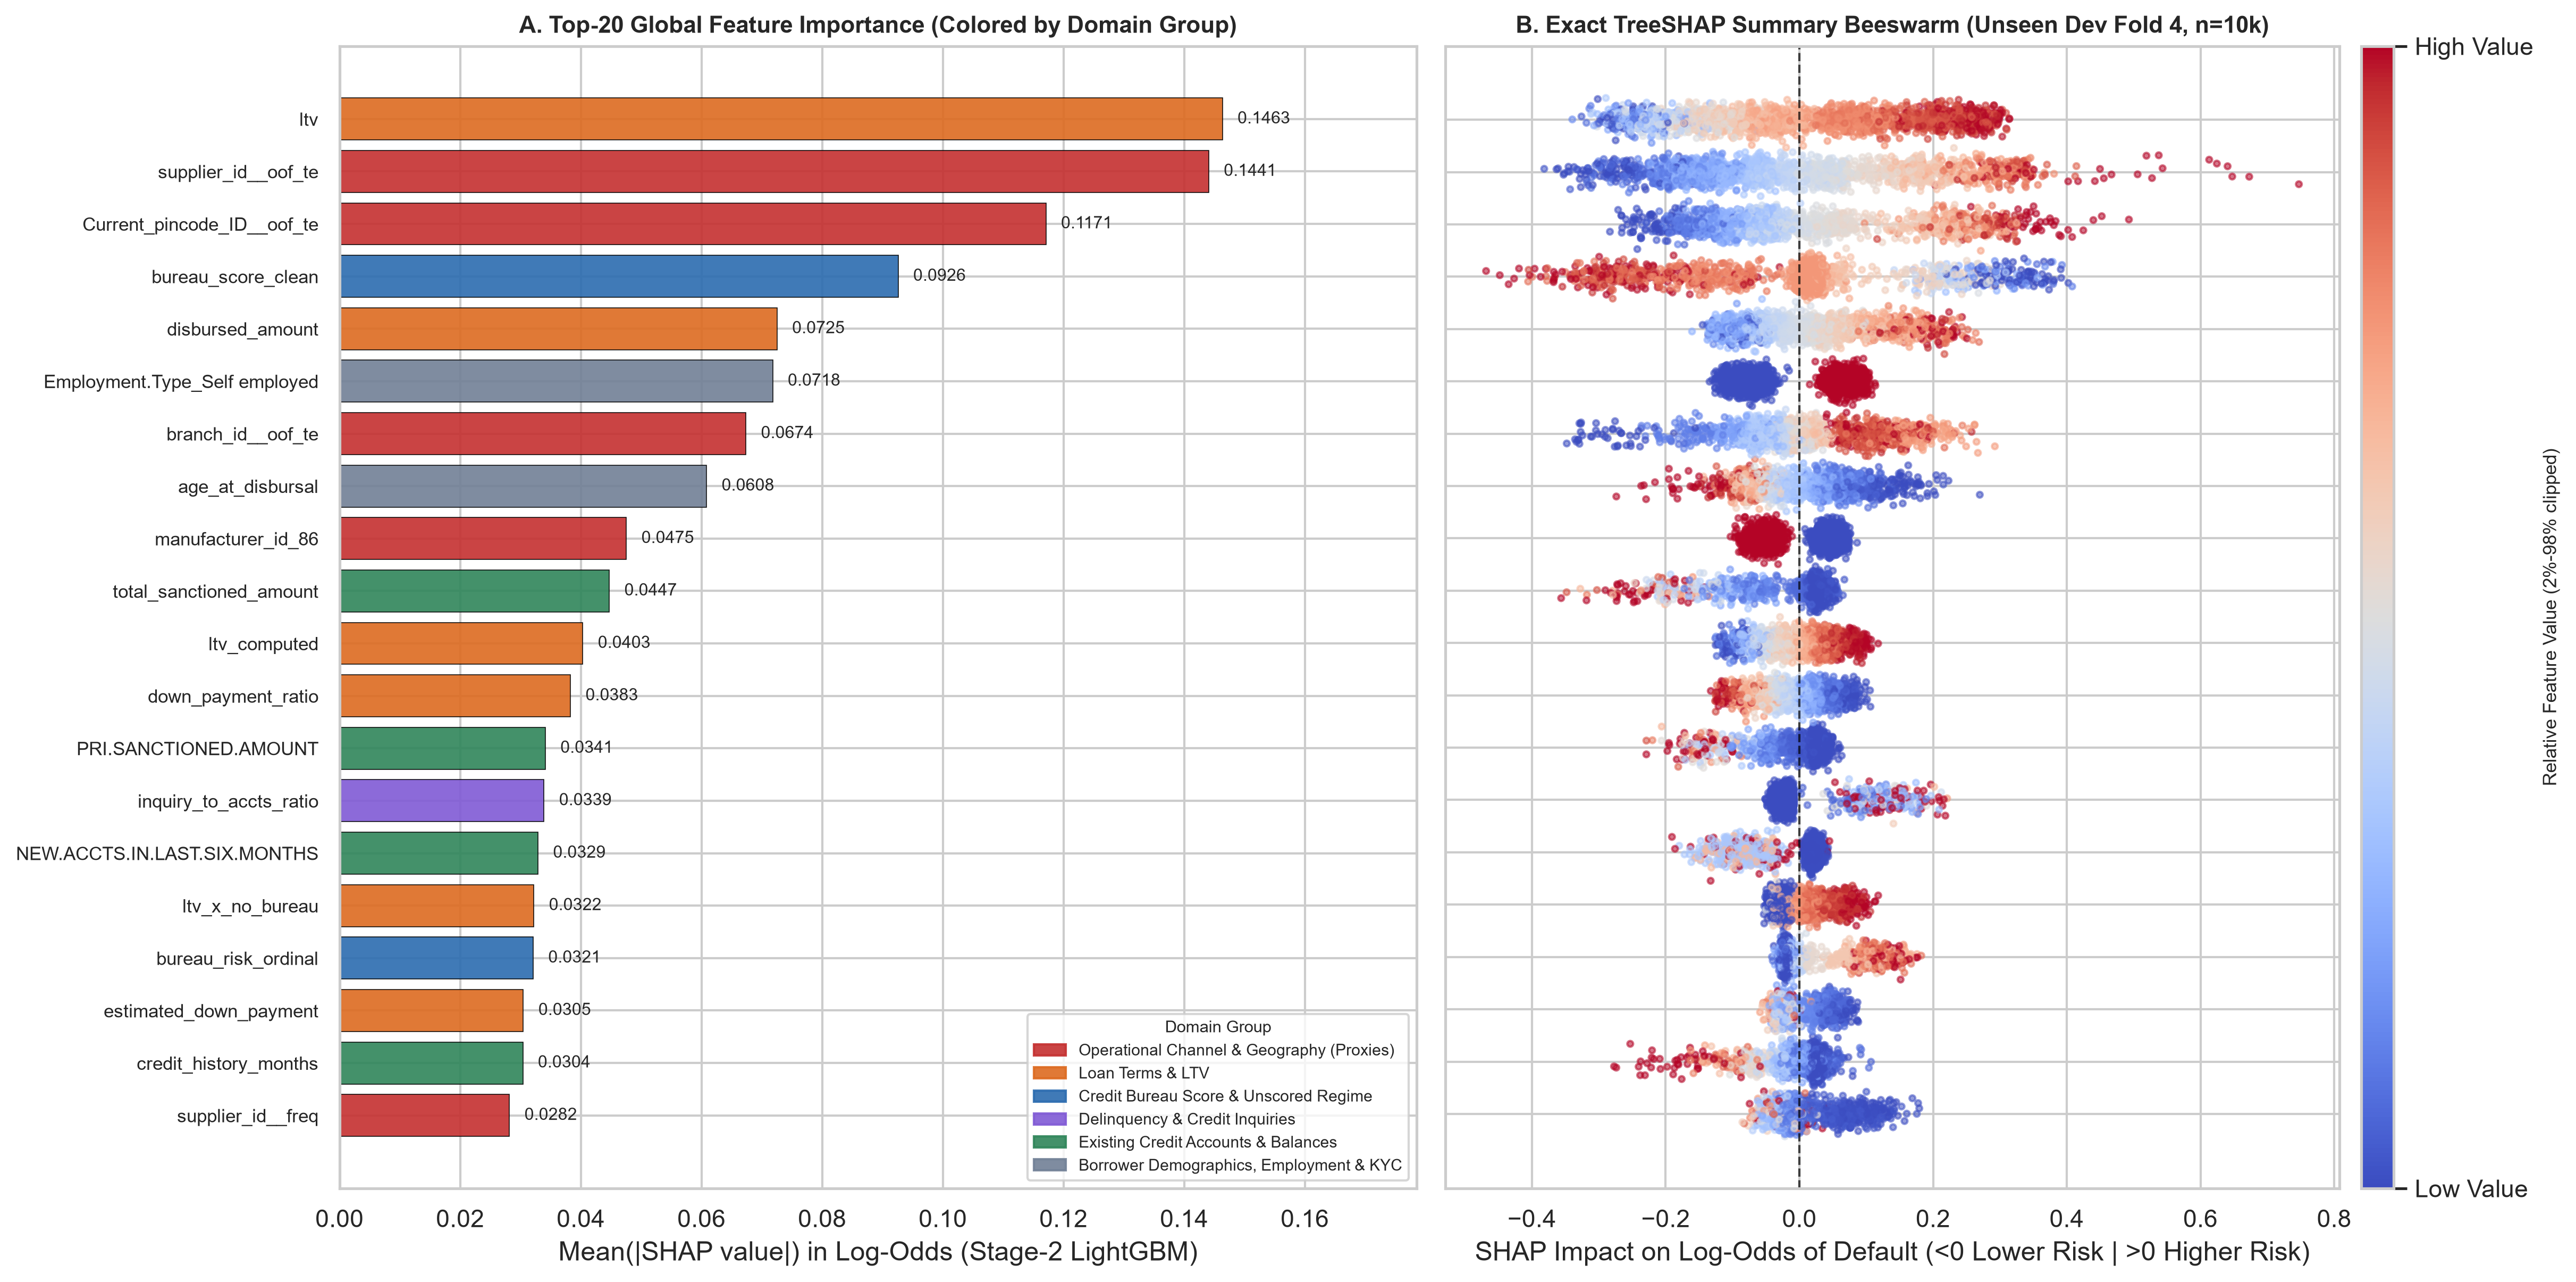
\includegraphics[width=0.95\textwidth]{figures/exp_01_shap_global_and_beeswarm.png}
  \caption{Top-20 global features ranked by mean $|\text{SHAP}|$ (left) and TreeSHAP beeswarm plot showing how high/low values shift default log-odds (right).}
  \label{fig:shap_global}
\end{figure}

Across the portfolio, operational channels and geography (\texttt{supplier\_id}, \texttt{branch\_id}, vehicle make, and \texttt{Current\_pincode\_ID}) account for $28.90\%$ of total OOT SHAP weight, followed by loan terms and LTV ($23.81\%$), existing credit accounts, recent openings, and balances ($19.39\%$), borrower demographics, employment, and KYC ($12.58\%$), delinquency history and inquiries ($7.76\%$), and numerical bureau scores ($7.55\%$). Key individual risk drivers align with domain finance intuition: higher \texttt{ltv} (especially above $75\%$), high-risk dealerships (\texttt{supplier\_id\_\_oof\_te}), weaker \texttt{bureau\_score\_clean} ($<620$), larger \texttt{disbursed\_amount}, \texttt{Self employed} status, younger borrower age, and recent credit inquiries all increase default risk. Exact pairwise SHAP analysis on XGBoost further confirms strong non-linear interactions between \texttt{disbursed\_amount} $\times$ \texttt{ltv} and between \texttt{ltv} $\times$ dealership/bureau scores.

\begin{figure}[htbp]
  \centering
  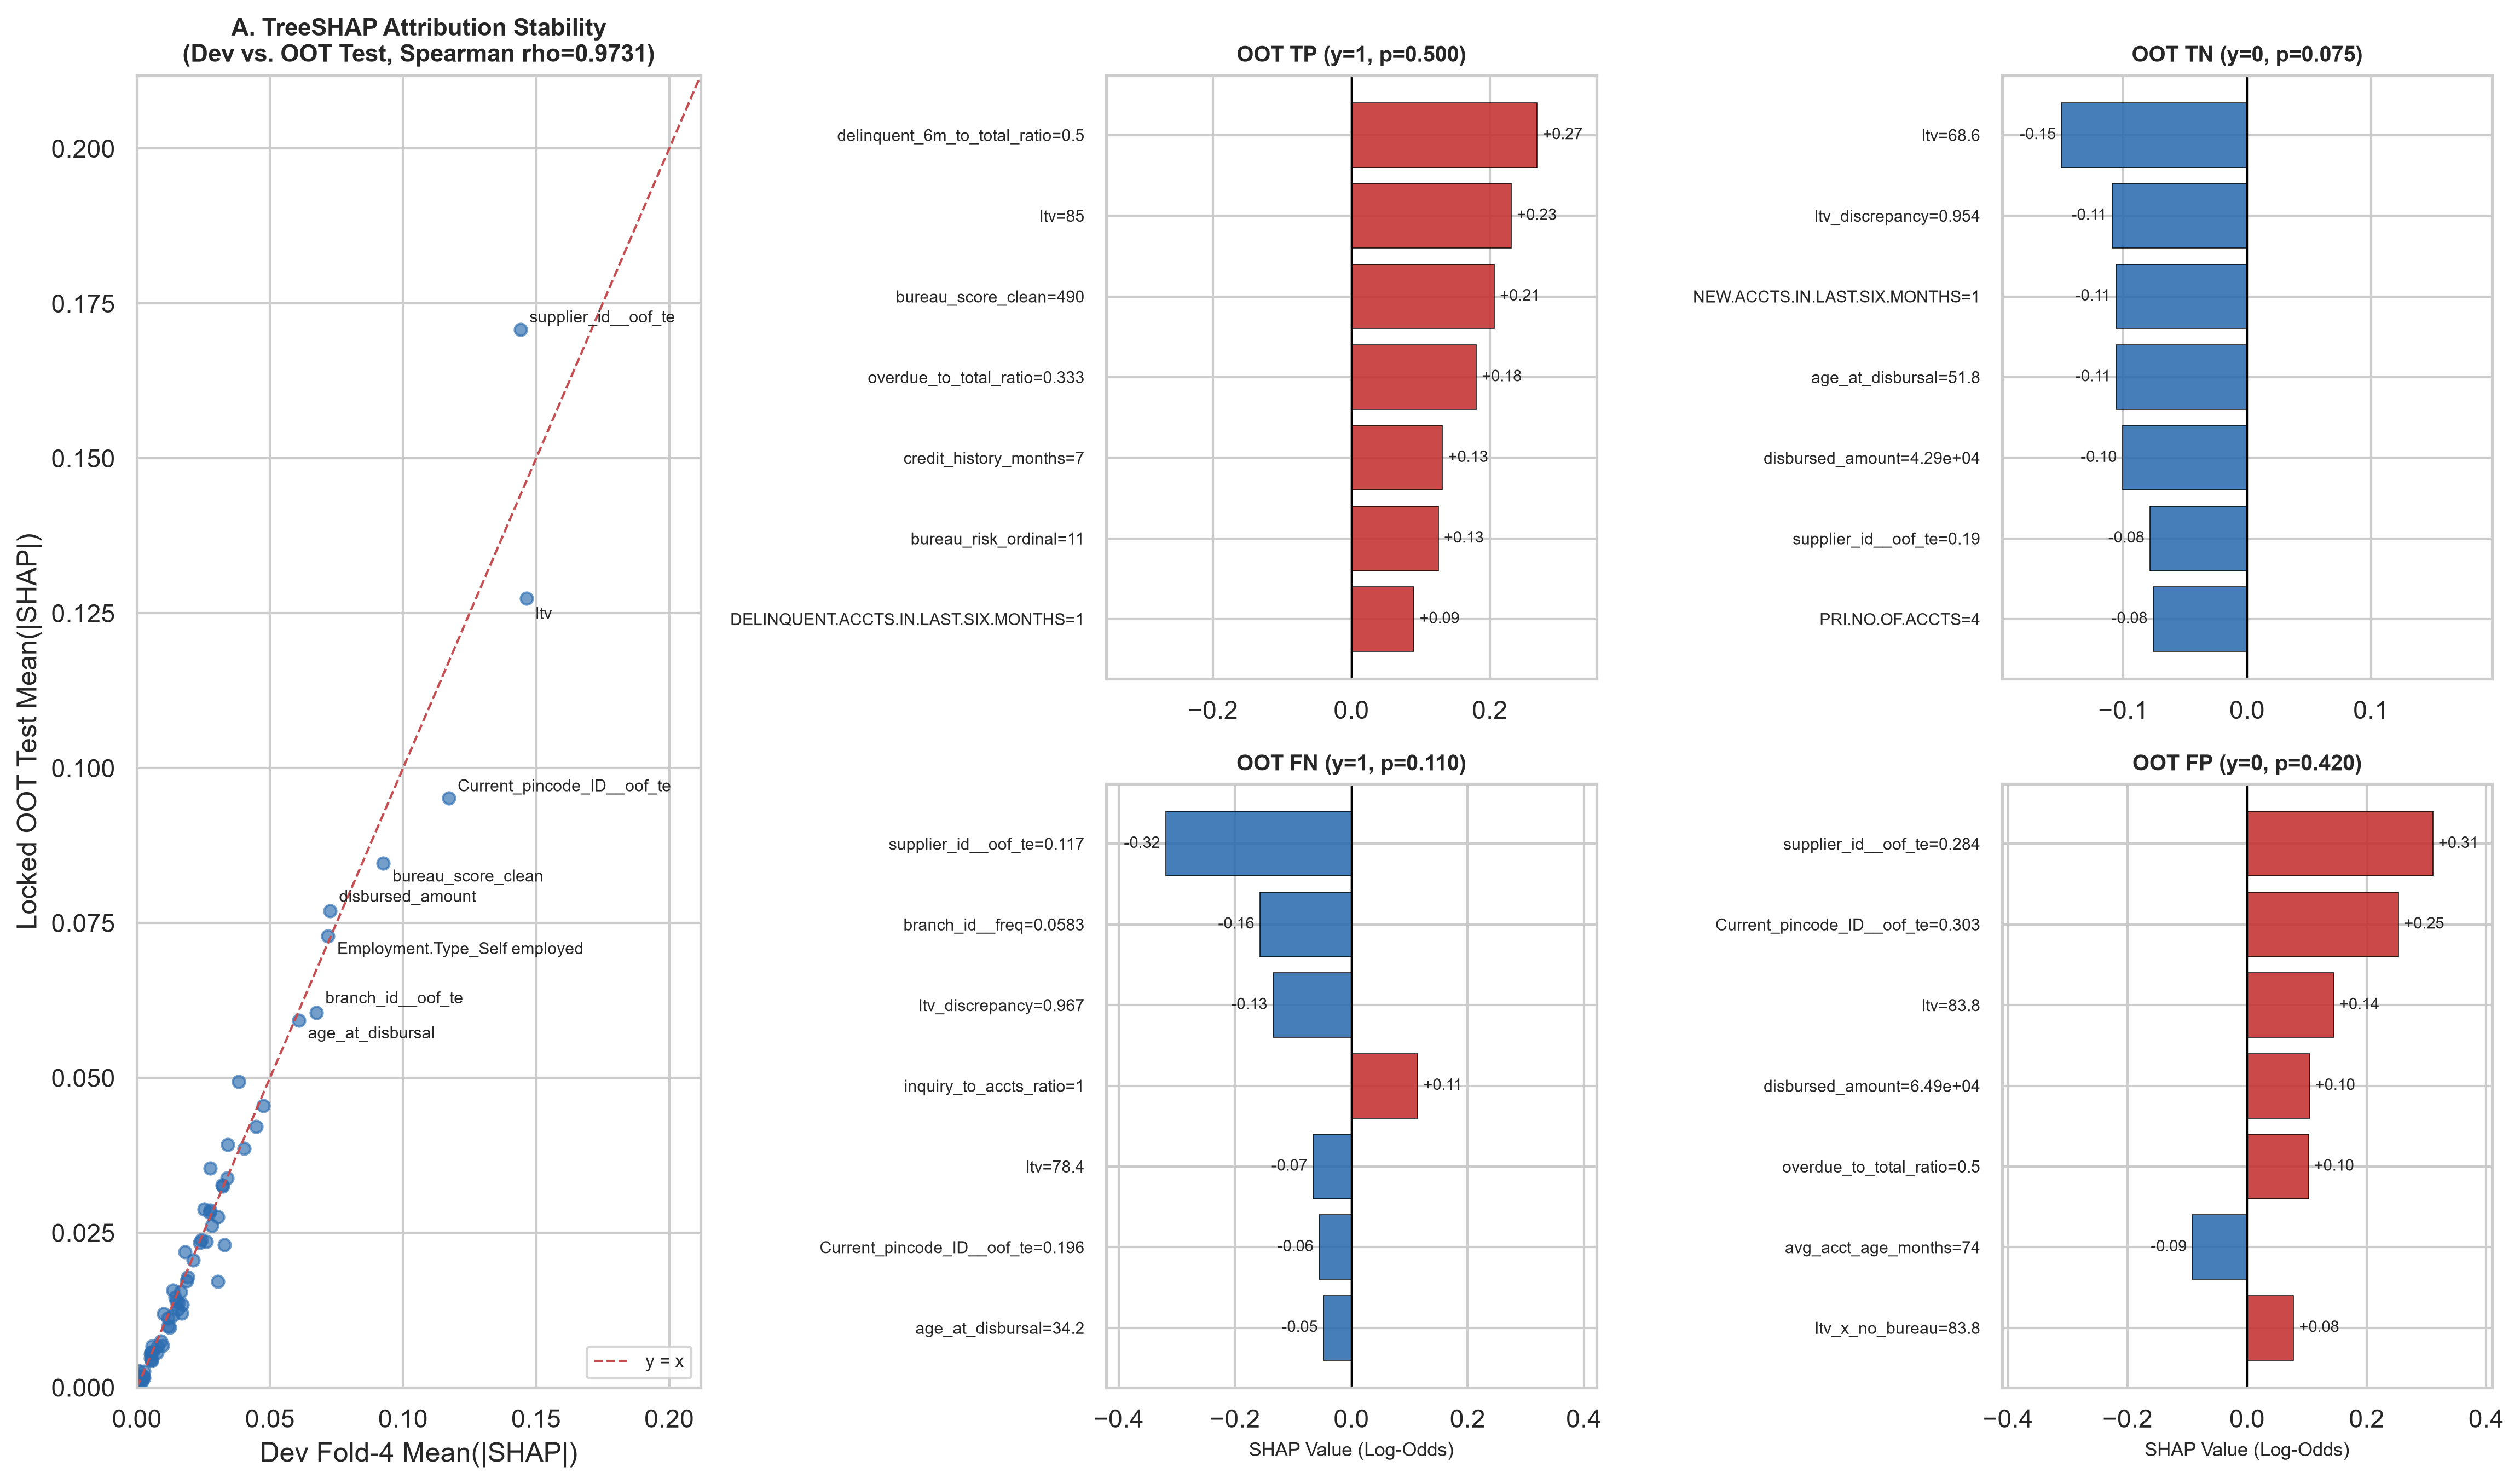
\includegraphics[width=0.95\textwidth]{figures/final_05_test_xai_stability_and_errors.png}
  \caption{Cross-time TreeSHAP importance stability between Development and OOT Test ($\rho = 0.973$, left) and four individual OOT explanation case studies (right).}
  \label{fig:shap_cases}
\end{figure}

Inspecting individual OOT cases (Figure~\ref{fig:shap_cases}, right) and subgroup cohorts reveals important operational nuances:
\begin{itemize}
  \item \textbf{Clear Successes (\texttt{TP 630094}, $\hat{p}=0.500$; \texttt{TN 645014}, $\hat{p}=0.075$):} The high-risk default case combines $85\%$ LTV, bureau score $490$, and recent 6-month delinquency, whereas the safe case pairs low leverage ($68.6\%$ LTV), solid credit score ($680$), and borrower maturity ($51.8$ years).
  \item \textbf{Thin-File Blind Spot (\texttt{FN 621929}, $y=1$, $\hat{p}=0.110$ vs.\ \texttt{FP 652048}, $y=0$, $\hat{p}=0.420$):} When an applicant has no bureau score ($0$), strong dealership/pincode priors heavily sway predictions---letting a risky thin-file loan slip past at a safe dealership (\texttt{supplier TE = 0.117}) while flagging a borrower who ultimately repaid (\texttt{FP 652048}) due to combined high dealership/pincode risk (\texttt{supplier TE = 0.284}, \texttt{pincode TE = 0.303}), $83.8\%$ LTV, and an overdue secondary guarantor account (\texttt{overdue\_to\_total\_ratio = 0.50}).
  \item \textbf{Subgroup Separation Gap:} Across OOT Test slices, LightGBM separates risk much better for borrowers with credit bureau scores ($\text{AUC} = 0.683$) than for unscored thin-file borrowers ($\text{AUC} = 0.645$, $-3.8\text{ percentage points}$), and performs stronger on mature borrowers aged $46+$ ($\text{AUC} = 0.694$) than ages $18\text{--}25$ ($\text{AUC} = 0.642$).
\end{itemize}

Because $59\%$ flagging is too broad for blanket automatic rejections and dealer proxies carry nearly $29\%$ SHAP weight, the champion model should operate inside a \textbf{Three-Tier Human-in-the-Loop Underwriting Policy}: (1) \textbf{Auto-Approve} ($\hat{p} < 0.167$, $\sim 41\%$ volume), adding an income-verification rule if a thin-file borrower seeks $>78\%$ LTV at a low-risk dealer; (2) \textbf{Manual Underwriting Review} ($0.167 \le \hat{p} < 0.317$, $\sim 44\%$ volume), where phone checks capture up to $75.6\%$ of defaults while protecting good applicants flagged by regional proxies; and (3) \textbf{Counter-Offer or Decline} ($\hat{p} \ge 0.317$, top $15\%$), requiring higher down payments supported by borrower-specific SHAP reason codes alongside periodic base-rate probability recalibration when seasonal risk shifts.
